\section{La sortie web}

\subsection{Introduction}

	Nous avons réalisés une sortie afin d'exploiter au mieux les données qui ont été créées par l'algorithme génétique. Le premier objectif de cette sortie web est surtout de pouvoir visualiser les données après leurs sortie, par la suite le but de cette sortie est de présenter une évolution des armées et ainsi remarquer le comportement de l'algorithme génétique.

\subsection{Disposition de la page web:}

	\subsubsection{Affichage de données générale}
	
		Cette page web sépare les combats par tournois afin de libérer de l'espace sur la page web est facilité la lecture des données. 
		
		\begin{figure}
			\center
			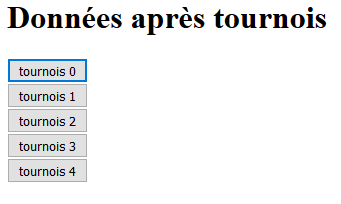
\includegraphics[scale=1]{webimg/index.PNG}
			\caption{la page au premier chargement} 
		\end{figure}
		
		Sur cette page l'utilisateur pourra cliquer sur le bouton afin d'afficher les information du tournois concerner, les données affichées sont les compositions initiales de chaque armées ainsi que leur score. Le score représente le nombre totale de victoire que l'armée à obtenue lors de ce tournois.
		
		\begin{figure}
			\center
			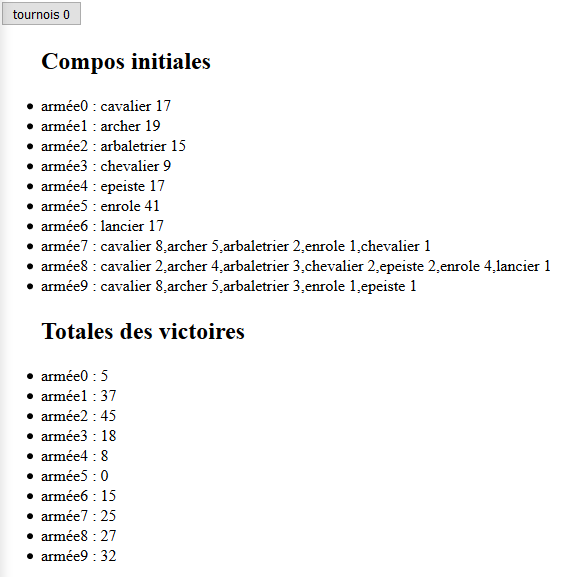
\includegraphics[scale=1]{webimg/but.png}
			\caption{la page après le clique sur un bouton tournois} 
		\end{figure}
		
		Ainsi via cette page web on peut remarquer si une certaine composition est meilleur qu'une autre. Pour cela il suffit de regarder la partie "Compos initiale". Si une armé ce répète plusieurs fois on peut alors juger qu'elle est optimisé.